%% ---------------------------------------------------------------------------------------------------------------------

\chapter{\textit{go-safer}: Detecting Unsafe Misuses}\label{ch:go-safer}

Another major contribution of this thesis is the development of \toolSafer{}, a \toolVet{}-style, open-source linter
tool with a focus on the \unsafe{} \acrshort{API} in Go.
It can identify some of the unsafe code patterns described in Chapter~\ref{ch:unsafe-security-problems} and thus help
developers to write safer code.
This chapter describes the design and implementation of \toolSafer{}, as well as an evaluation of its effectiveness both
using the labeled data set of \unsafe{} usages presented in the previous chapter and a manual analysis of \checkNum{six}
open-source Go packages.

\begin{figure}[htp!]
    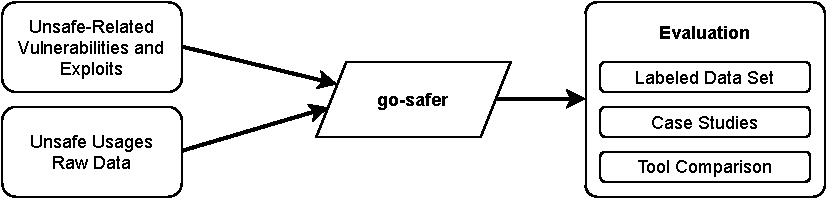
\includegraphics[width=\textwidth]{assets/figures/chapter5/outline5.pdf}
    \caption{Role of Chapter 5 in the thesis outline}
    \label{fig:outline5}
\end{figure}



%% ---------------------------------------------------------------------------------------------------------------------

\section{Design}\label{sec:go-safer:design}

The \toolSafer{} static analysis tool is designed as a linter to detect two misuses of the \unsafe{} \acrshort{API}.
The first is the incorrect conversion pattern between slices and strings by creating their header structures as
composite literals as described in Sections~\ref{subsec:unsafe-security-problems:slice-casts:gc-race}
and~\ref{subsec:unsafe-security-problems:slice-casts:escape-analysis}.
The second is a direct conversion between struct types containing incompatible types with architecture-dependent sizes.
The source code and documentation of \toolSafer{} is available on
\github{}\footnote{\url{https://github.com/jlauinger/go-safer}}.

\begin{lstlisting}[language=Golang, float, label=lst:go-safer-sliceheader-pass, caption=First vulnerable code pattern detected by \toolSafer{}]
func unsafeFunction(s string) []byte {
    sH := (*reflect.StringHeader)(unsafe.Pointer(&s))
    bH := &reflect.SliceHeader{
        Data: sH.Data,
        Len:  sH.Len,
        Cap:  sH.Len,
    }
    return *(*[]byte)(unsafe.Pointer(bH))
}
\end{lstlisting}


\begin{lstlisting}[language=Golang, label=lst:go-safer-structcast-pass, caption=Second vulnerable code pattern detected by \toolSafer{}]
type A struct {
    x int
}
type B struct {
    y int64
}
func unsafeFunction(a A) B {
    return *(*B)(unsafe.Pointer(&a))
}
\end{lstlisting}


Usage: \textit{go-safer ./my/package}

\begin{figure}[htp!]
    %\vspace{2mm}
    \centering
    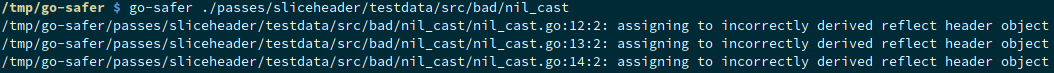
\includegraphics[width=\textwidth]{assets/images/chapter5/go-safer-screenshot.png}
    \caption{Usage example screenshot of \toolSafer{}}
    \label{fig:go-safer-screenshot}
    %\vspace{-14pt}
\end{figure}



%% ---------------------------------------------------------------------------------------------------------------------

\section{Implementation}\label{sec:go-safer:implementation}

\begin{figure}[!t]
    \vspace{2mm}
    \centering
    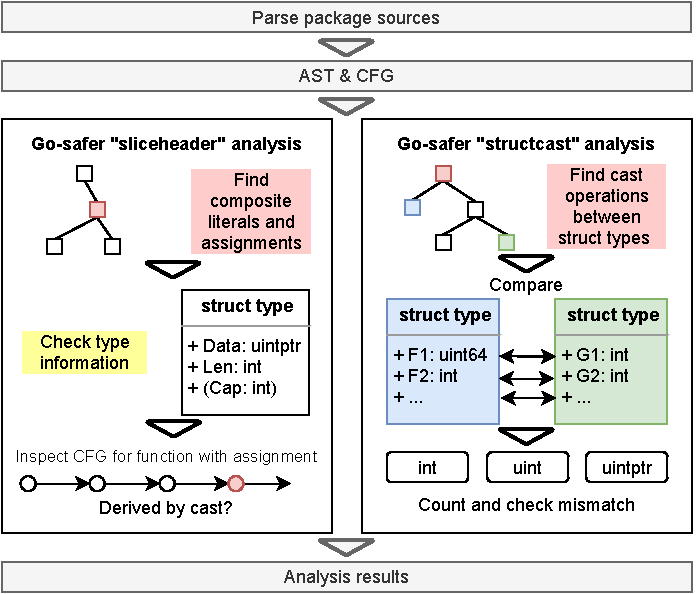
\includegraphics[width=0.48\textwidth]{gfx/figures/go-safer-architecture.pdf}
    %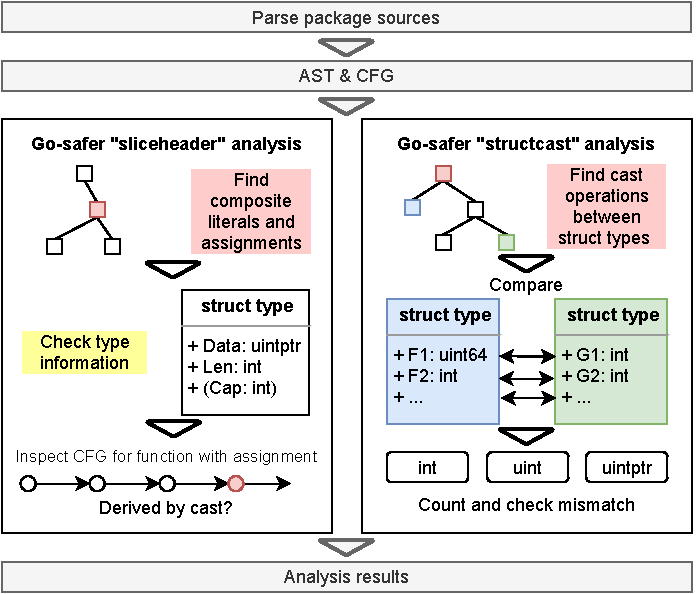
\includegraphics[width=0.45\textwidth]{gfx/figures/go-safer-architecture.pdf}
    \caption{Architecture of \toolSA{} static code analysis tool}
    \label{fig:safer-architecture}
    %\vspace{-14pt}
\end{figure}


Go vet analysis pass infrastructure
Low-level details
Verification with tests


%% ---------------------------------------------------------------------------------------------------------------------

\section{Evaluation}\label{sec:go-safer:evaluation}


%% ---------------------------------------------------------------------------------------------------------------------

\subsection{Labeled Usages}\label{subsec:go-safer:evaluation:labeled-usages}

Precision, Recall, calculated using manually labeled usages data set

\begin{table}[htp!]
    \centering
    \caption{Evaluation results for \toolSafer{} on the labeled data set of \unsafe{} usages}
    \label{tbl:gosafer-evaluation-dataset}
    \begin{tabular}{l||r|r|r|r||l|l|l|l}
        \textbf{Tool} & \textbf{TP} & \textbf{FP} & \textbf{TN} & \textbf{FN} & \textbf{Precision} & \textbf{Recall} & \textbf{Accuracy} & \textbf{F1-Score} \\
        \hline
        go-safer &   29   &    1   &   13   &    1   &   0.967       &  0.967     &    0.955     & 0.967  \\
        go vet   &    0   &    0   &   14   &   30   &   -           &  0         &    0.318     & 0      \\
        gosec    &   29   &   13   &    1   &    1   &   0.690       &  0.967     &    0.681     & 0.805  \\
    \end{tabular}
\end{table}


%% ---------------------------------------------------------------------------------------------------------------------

\subsection{Case Studies}\label{subsec:go-safer:evaluation:case-studies}

Manual inspection of some projects, used to calculate precision / recall of go-safer

\begin{table}[htp!]
    \centering
    \caption[Evaluation results for \toolSafer{} on manually analyzed packages packages]
        {Evaluation results for \toolSafer{} on manually analyzed packages packages~\newline \tiny ~\newline \footnotesize
        Tools: \underline{a} \toolSafer{}, \underline{b} \toolVet{}, \underline{c} \toolGosec{} \tiny ~\newline}
    \label{tbl:go-safer-evaluation-packages}
    \begin{adjustbox}{max width=\textwidth}
        \begin{tabular}{l||rrr|rrr|rrr|rrr||lll|lll|lll|lll}
            \textbf{Package} & \multicolumn{3}{c|}{\textbf{TP}}                & \multicolumn{3}{c|}{\textbf{FP}}                   & \multicolumn{3}{c|}{\textbf{TN}}                    & \multicolumn{3}{c||}{\textbf{FN}}                  & \multicolumn{3}{c|}{\textbf{Precision}}  & \multicolumn{3}{c|}{\textbf{Recall}}    & \multicolumn{3}{c|}{\textbf{Accuracy}}           & \multicolumn{3}{c}{\textbf{F1-Score}}    \\
            {}               & \textit{a}            & \textit{b} & \textit{c} & \textit{a}             & \textit{b} & \textit{c}   & \textit{a}            & \textit{b}   & \textit{c}   & \textit{a}             & \textit{b}  & \textit{c}  & \textit{a}     & \textit{b} & \textit{c} & \textit{a}    & \textit{b} & \textit{c} & \textit{a}     & \textit{b}     & \textit{c}     & \textit{a}     & \textit{b} & \textit{c} \\
            \hline
            v1               & 0                     & 0          & 0          & 0                      & 0          & 676          & 677                   & 677          & 1            & 0                      & 0           & 0           & -              & -          & 0          & -             & -          & -          & 1              & 1              & 0.001          & -              & -          & -          \\
            \rowcolor{verylightgray}
            native           & 48                    & 0          & 0          & 9                      & 0          & 98           & 101                   & 110          & 12           & 0                      & 48          & 48          & 0.842          & -          & 0          & 1             & 0          & 0          & 0.943          & 0.696          & 0.076          & 0.914          & -          & -          \\
            socket           & 0                     & 0          & 0          & 0                      & 0          & 16           & 115                   & 115          & 99           & 0                      & 0           & 0           & -              & -          & 0          & -             & -          & -          & 1              & 1              & 0.861          & -              & -          & -          \\
            \rowcolor{verylightgray}
            ebpf             & 0                     & 0          & 0          & 1                      & 0          & 38           & 64                    & 65           & 27           & 0                      & 0           & 0           & 0              & -          & 0          & -             & -          & -          & 0.985          & 1              & 0.415          & -              & -          & -          \\
            label            & 0                     & 0          & 0          & 0                      & 0          & 7            & 8                     & 8            & 1            & 0                      & 0           & 0           & -              & -          & 0          & -             & -          & -          & 1              & 1              & 0.125          & -              & -          & -          \\
            \rowcolor{verylightgray}
            jlexer           & 1                     & 0          & 0          & 0                      & 0          & 2            & 4                     & 4            & 2            & 0                      & 1           & 1           & 1              & -          & 0          & 1             & 0          & 0          & 1              & 0.8            & 0.4            & 1              & -          & -          \\
            \hline
            \textbf{Total}   & \textbf{49}           & \textbf{0} & \textbf{0} & \textbf{10}            & \textbf{0} & \textbf{837} & \textbf{969}          & \textbf{979} & \textbf{142} & \textbf{0}             & \textbf{49} & \textbf{49} & \textbf{0.831} & \textbf{-} & \textbf{0} & \textbf{1}    & \textbf{0} & \textbf{0} & \textbf{0.990} & \textbf{0.952} & \textbf{0.138} & \textbf{0.907} & \textbf{-} & \textbf{-} \\
        \end{tabular}
    \end{adjustbox}
\end{table}


%% ---------------------------------------------------------------------------------------------------------------------

\subsection{Comparison with Existing Tools}\label{subsec:go-safer:evaluation:linters-comparison}

Go vet / Gosec
